\documentclass[pdftex,12pt,a4paper]{article}

\usepackage{graphicx}  
\usepackage[margin=2.5cm]{geometry}
\usepackage{breakcites}
\usepackage{indentfirst}
\usepackage{pgfgantt}
\usepackage{pdflscape}
\usepackage{float}
\usepackage{epsfig}
\usepackage{epstopdf}
\usepackage[cmex10]{amsmath}
\usepackage{stfloats}
\usepackage{multirow}

\renewcommand{\refname}{REFERENCES}
\linespread{1.3}

\usepackage{mathtools}
%\newcommand{\HRule}{\rule{\linewidth}{0.5mm}}
\thispagestyle{empty}
\begin{document}
\begin{titlepage}
\begin{center}
\textbf{}\\
\textbf{\Large{ISTANBUL TECHNICAL UNIVERSITY}}\\
\vspace{0.5cm}
\textbf{\Large{COMPUTER ENGINEERING DEPARTMENT}}\\
\vspace{2cm}
\textbf{\Large{BLG 222E\\ Computer Organization \\ Project 1}}\\
\vspace{2.8cm}
\begin{table}[ht]
\centering
\Large{
\begin{tabular}{lcl}
\textbf{PROJECT DATE}  & : & 12.04.2023\\
\end{tabular}}
\end{table}
\vspace{1cm}
\textbf{\Large{GROUP MEMBERS:}}\\
\begin{table}[ht]
\centering
\Large{
\begin{tabular}{rcl}
number  & : & name \\
150220762  & : & Muhammed Yusuf Mermer  \\
150210071  & : & Emre Çamlıca \\
\end{tabular}}
\end{table}
\vspace{2.8cm}
\textbf{\Large{SPRING 2023}}

\end{center}

\end{titlepage}

\thispagestyle{empty}
\addtocontents{toc}{\contentsline {section}{\numberline {}FRONT COVER}{}}
\addtocontents{toc}{\contentsline {section}{\numberline {}CONTENTS}{}}
\setcounter{tocdepth}{4}
\tableofcontents
\clearpage

\setcounter{page}{1}
\section{INTRODUCTION}


\section{IMPLEMENTATIONS AND EXPLANATIONS }
\subsection{Part 2}
\subsubsection{Part 2.c}
In part 2c, we implemented Adress Register File (ARF) using registers we implemented at 
very begining. As a parameter values, we gave registers 8 bits as 8 bit is necesarry for 
implementing PC, AR, SP and PCPast. Besides, of enable and clock these registers 
already supports funsel and load capabilities, which works as specified in part 2.a. 
Therefore, we can directly send clock, funsel and load informations coming from 
input of this module to these registers without writing them again explicitly.

However, for the rsel, like in the part 2.b we will send individual bits to the enables of
the registers. As in the insturction, if a bit comming to the enable is 1, then operation
decleared by funsel will be done.

All 8-bit of information coming from these registers are connected to 16 multiplexers.

First 8 of them used for getting result of outA and other 8 used for getting result of 
outB. Which of these groups takes inputs with same patterns.

What these multipexers do is that they take significatly same digits of different registers 
as inputs and output the bit of a register that wanted by outasel or outbsel. As specified
in the part 2.c; 00 gives AR's bits,01 SP's bits, 10 PCPrev's bits,11 PC's bits. 
These two 8 bits comming from multipexers concatinated in outa and outb and gaved as
the output of the module.

\textbf{inputs:}    clk(1 bit),
load(8 bits),
outasel(2 bits),
outbsel(2 bits),
funsel(2 bits),
rsel(4 bits)

\textbf{outputs:}    
outa(8 bits),
outb(8 bits)

\textbf{module name:} arf

\subsection{Part 3}
I designed the required functions of the ALU for each FunSel case. The functions corresponding to each case will be discussed in the
sub-sections. I defined 4 extra variables that made it easier to design the arithmetic functions. These variables are basically the 9 
bit representations of $A, B, \overline{B}$ and the result $"out"$ of the corresponding arithmetic operation, with the 9'th bits of 
$A, B$ and $\overline{B}$ set to 0 to correctly represent arithmetic  operations using 8 bits in verilog. 
\newline
I used an always block to be able to change outputs whenever a different input is given and inside of it, I used "case" statement to
give the outputs corresponding to each Funsel input. The registers are never reset and their states change only when they are allowed
to. 
\newline
Before explaining each funsel case, I will talk about the certain patterns I use to check N, Z and C flags whenever it is necessary. 
For the N flag, I assign the most significant bit of the OutALU to Flag[1], which indicates the sign bit of a binary number. 
For the Z flag, I check whether the OutALU is compoesed of full of 0's. For the C flag in arithmetic operations I check the most 
significant bit of the out variable, which is a 9 bit register to store the result of arithmetic operations; in shift operations I 
check the dissapearing bits of A after doing the shift operation. That is, the most significant bit for the right shift and the 
least significant one for the left shift. 
Checking the overflow flag is basically done by checking the changes in the most significant bit. I will discuss each of them
in the following sub-sections, as it is done differently for each operation. 

\subsubsection{FunSel=0000}
OutALU is assigned to $A$, then the necessary flags are set.
\subsubsection{FunSel=0001}
OutALU is assigned to $B$, then the necessary flags are set.
\subsubsection{FunSel=0010}
OutALU is assigned to $\overline{A}$, then the necessary flags are set.
\subsubsection{FunSel=0011}
OutALU is assigned to $\overline{B}$, then the necessary flags are set.
\subsubsection{FunSel=0100}
The result of the addition of 9 bit versions of $A$ and $B$ is assigned to the 9 bit variable $out$. The carry flag is checked 
afterwards, if it is 1, the $out$ is incremented by one. After that the necessary flags are set.
\newline
When adding two binary numbers an overflow can occur only when the two numbers have the same sign, denoted by $A[7]\land B[7]$. 
We can understand that an overflow occured when the result is different than the signs of the operands. We can logically express this 
condition as $(A[7]\land B[7])\oplus {OutALU[7]}$, a logic one result indicating that an overflow occured.
\subsubsection{FunSel=0101}
The result of the addition of 9 bit versions of $A$ and $\overline{B}$ is assigned to the 9 bit variable $out$ with the addition of
binary 1. After that the necessary flags are set.
\newline
When subtracting two binary numbers an overflow can occur only when the two numbers have different signs, denoted by $A[7]^B[7]$.
We can understand that an overflow occured when the result is different than the sign of the first operand, A, since subtracting 
a number with a different sign should always result in a number having the same sign as the first operand. We can denote this 
condition by $A[7]\oplus {OutALU[7]}$. We can combine the two logic expressions we formed by "and"ing them to create a logic expression 
for overflow, which can be written as $(A[7]\oplus {B[7]})\land(A[7]\oplus {OutALU[7]})$, a logic one result indicating that an 
overflow occured. 
\subsubsection{FunSel=0110}
For the "compare" function, the "subtraction" operation explained in the previous sub-section is used with the corresponding flags.
However this time the result of the subtraction is interpreted considering the flags to give the required output.
The function interprets the result using if/else statements. In the if statements the possible cases indicating $A>B$ are checked
and the OutALU is set as A if the condition is true, else OutALU is set as full of 0's.
\newline
The first possibility indicating $A>B$ is that there is no overflow, the result is not negative and it is not zero, implying that
$A-B>0$. This is denoted by the logic expression $\overline{Flag[0]}\land\overline{Flag[1]}\land\overline{Flag[3]}$.
\newline
The second possibility indicating $A>B$ is that there is overflow and A is positive. Which implies that B is negative. 
This is denoted by the logic expression $Flag[0]\land\overline{A[7]}$.
\newline
All other combinations of flag outputs imply that either $B>A$ or $A=B$, which will result in a 0 output.
\subsubsection{FunSel=0111}
The result of the "bitwise and" operation on A and B is assigned to OutALU, then the necessary flags are set. 
\subsubsection{FunSel=1000}
The result of the "bitwise or" operation on A and B is assigned to OutALU, then the necessary flags are set. 
\subsubsection{FunSel=1001}
The result of the "bitwise nand" operation on A and B, done by negating every bit of $A\land B$ is assigned to OutALU, then the 
necessary flags are set. 
\subsubsection{FunSel=1010}
The result of the "bitwise xor" operation on A and B is assigned to OutALU, then the necessary flags are set. 
\subsubsection{FunSel=1011}
The result of "logic shift left" operation by 1 bit on A is stored in OutALU. After that the necesarry flags are set. 
\subsubsection{FunSel=1100}
The result of "logic shift right" operation by 1 bit on A is stored in OutALU. After that the necesarry flags are set. 
\subsubsection{FunSel=1101}
The result of "logic shift left" operation by 1 bit on A is stored in OutALU. After that the necesarry flags are set.
\newline
Here, if The most significant bit of OutALU is not the same as that of $A$'s an overflow flag is raised. This is denoted by the logic
expression $A[7]\oplus{OutALU[7]}$, a logic 1 result indicating that an overflow occured.
\subsubsection{FunSel=1110}
The result of "logic shift right" operation by 1 bit on A is stored in OutALU. Then, the most significant bit of OutALU is set 
equal to the most significant bit of $A$ as expected to prevent overflow. After that the zero flag is set.
\subsubsection{FunSel=1111}
The result of "logic shift right" operation by 1 bit on A is stored in OutALU. The least significant bit of $A$ is assigned to the 
most significant bit of OutALU so that the circular shift is done correctly. After that the necesarry flags are set. 

\subsubsection{}
\textbf{inputs:}  
A(8 bits),
B(8 bits),
Funsel(4 bits)

\textbf{outputs:}    
Flag(4 bits),
OutALU(8 bits)

\textbf{module name:} alu

\subsection{Part 4}
In this part, our purpose is to combine all previously made modules. 
At first we started with adding memory module that provided. We see that when 
we are in the write mode it gives high impedance as output and in the read mode
 we cannot change what is inside of memory.

 Our first thought about this is we will write a test bench, so that IR will not
  take input from memory when memory is in the write mode. Not only IR but also 
  two Multiplexer is also taking input from memory which we want to avoid when 
  memory is in writing mode. We did not implemeted our test bench because we saw
   that test bench is already shared one day later (the day we were thinking to 
   start implemeting).

   After adding module of memory, we defined wires that comes into/ goes out of 
   memory. Adress and outALU is not currently output of any other module. 

   At first we did not thought that nearly every wires have to be senesed as 
   output as test bench required. Therefore, initally we made them as intermadiate 
   wires. Then after we see the output wire names, we changed nearlly all our wires' 
   name and make them output.

	For the connection of IR, we gave 8 least signficant bits to the Multiplexer A.
	At our initial design we output IR's most signficant 8 bits from system but later we change
	 it so that it outputs all 16 bits as outputs.

	After IR, we add modules of Multiplexer A and Multiplexer B. Even though 
	Multiplexer is already implemented for previous parts, we cannot use them 
	directly because they are just 1 bit which in case of use, make our module
	complicated. Hence, we made another module for four to one Multiplexer which 
	takes and gives 8 bit values. Not only four two one multiplexer, but also two
	to one multiplexer which also processing 8 bit values had been made to use on 
	multiplexer C. 

	After connecting relevant wires to multiplexers, we added ARF to the system.
	We add new inputs to the system so that we can modify outputs of the ARF.

	With the addition of this module we see that order of call of modules inside of another 
	module does not important if there is exist intermadiate signals (wires), because
	ARF depends on memory via multiplexer and memory depends on ARF through memory
	 address information.

	 Later we add register file and multipexer C to the system. And we made the connections.

	For the ALU at first we make sepearated flag register but due to input and outputs of ALU 
	is strictly given, we connot write sepearated cin input for ALU which directed us to use a register
	inside of ALU module for flag. Then we made proper input and output connections to the ALU
	module.

	


	\textbf{inputs:}
	ARFOutASel(2 bit), ARFOutBSel(2 bit), IRFunsel(2 bit), ARFFunSel(2 bit),
	RFFunSel(2 bit), ALUFunSel(4 bit), RFRSel(4 bit), ARFRSel(4 bit),
	Clock(1 bit), MemWR(1 bit), MemCS(1 bit), IREnable(1 bit),
	IRLH(1 bit), MuxASel(2 bit), MuxBSel(2 bit), MuxCSel(1 bit),
	RFOutASel(3 bit), RFOutBSel(3 bit), RFTSel(4 bit)


	\textbf{outputs:} 
	AOut (8 bits),
    BOut (8 bits),
    ALUOut (8 bits),
    ALUOutFlag (4 bits),
    ARFAOut (8 bits),
    Address (8 bits),
    MemoryOut (8 bits), 
    MuxAOut (8 bits), 
    MuxBOut (8 bits),
    MuxCOut (8 bits),
    IROut (16 bits)

	\textbf{module name:} ALUSystem







\section{DESIGN PHOTOS}
\subsection{Part 2}
\subsubsection{Part 2.c}
\begin{figure}[H]
	\centering
	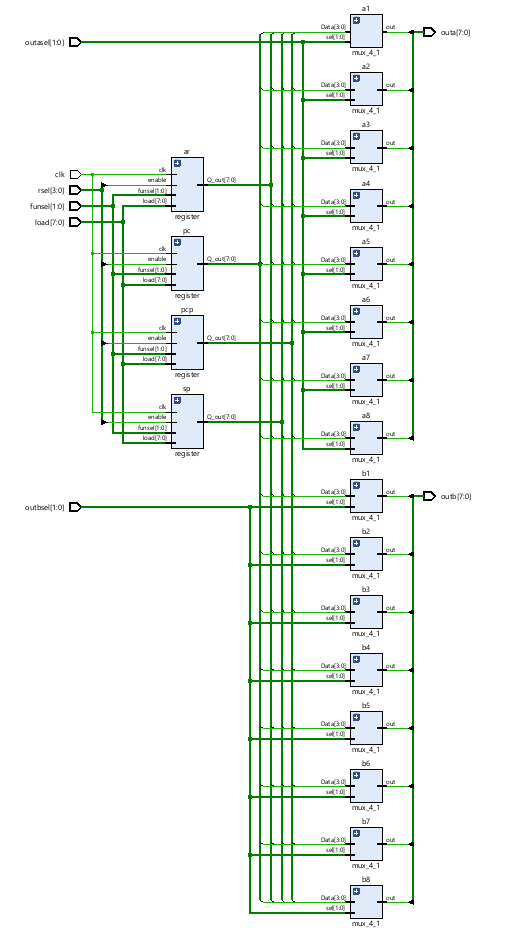
\includegraphics[width=0.5\textwidth]{design/arf.png}	
	\caption{ARF System Design}
	\label{ARF System Design}
\end{figure}

\subsection{Part 3}
\begin{figure}[H]
	\centering
	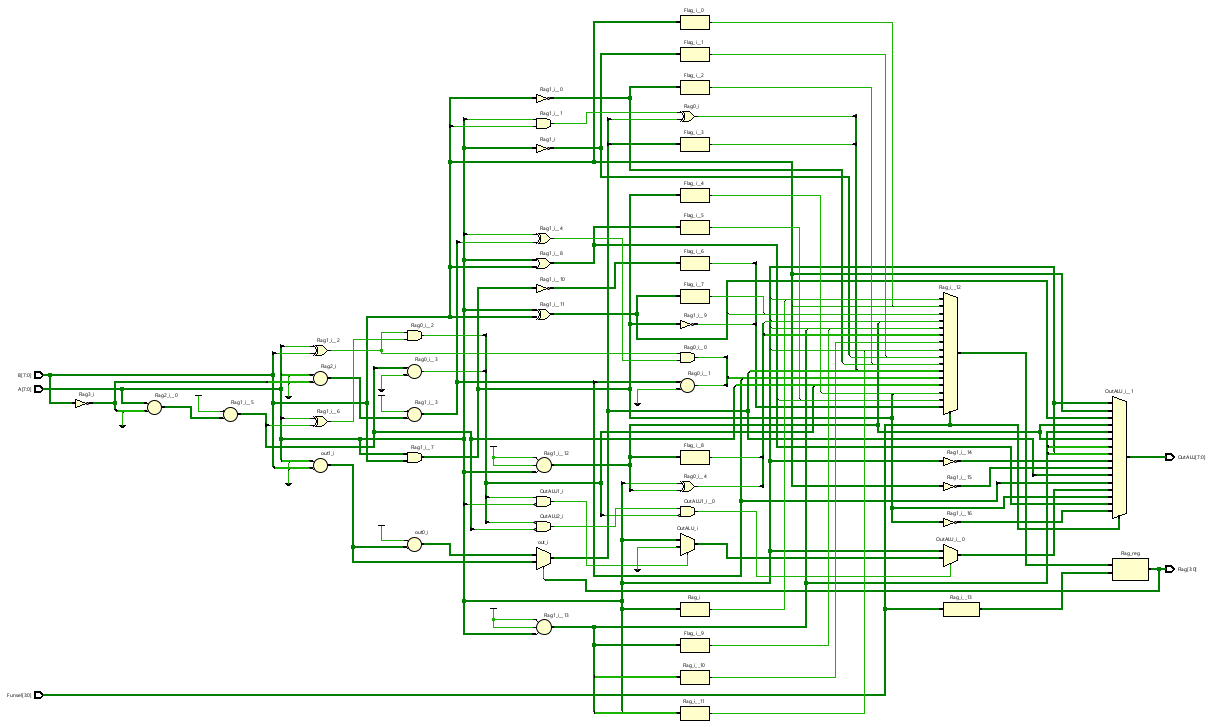
\includegraphics[width=0.5\textwidth]{design/alu.png}	
	\caption{ALU Design}
	\label{ALU Design}
\end{figure}

\subsection{Part 4}
    \begin{figure}[H]
    	\centering
    	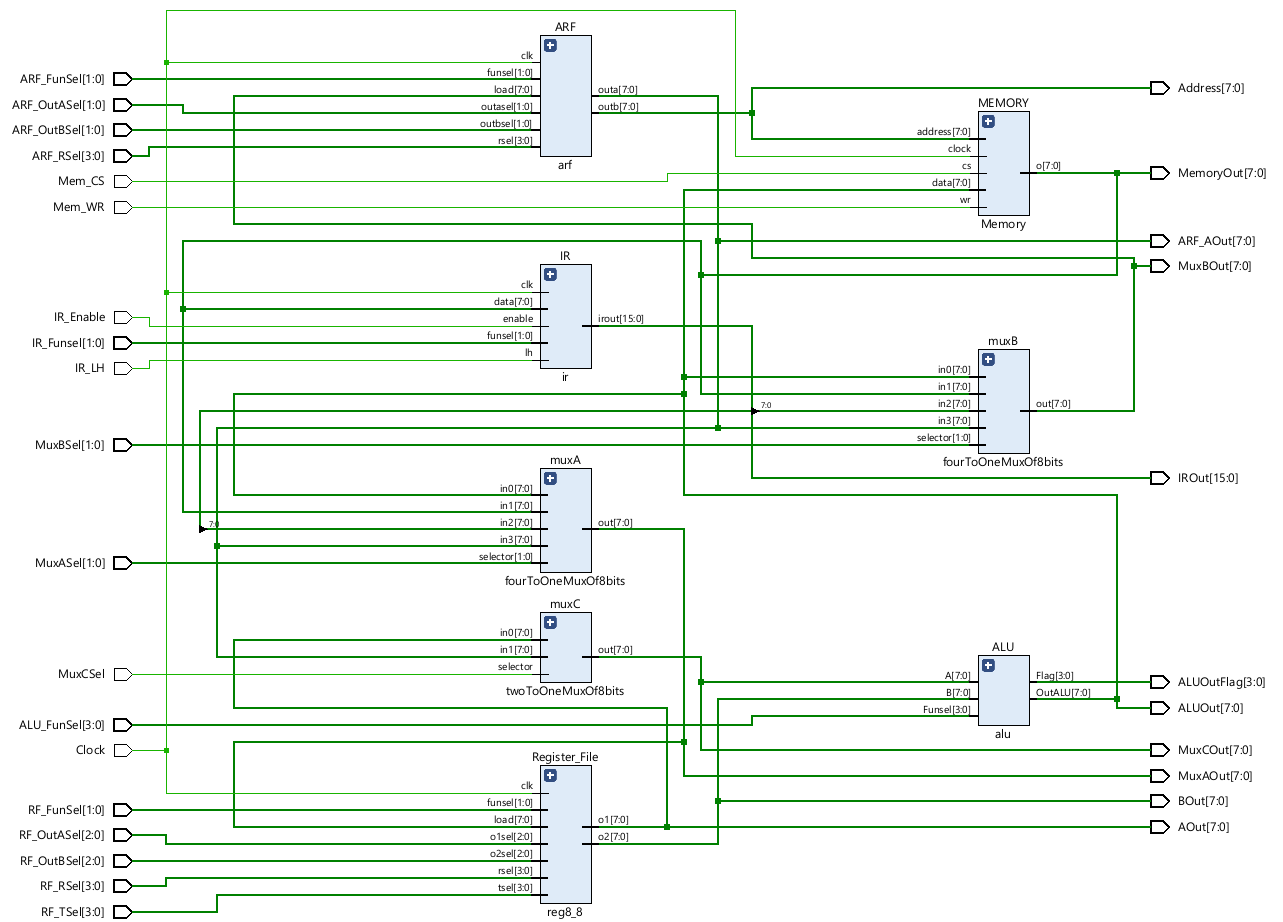
\includegraphics[width=0.9\textwidth]{design/ALU_system.png}	
    	\caption{ALU System Design}
    	\label{ALU System Design}
    \end{figure}








\section{RESULTS}
\subsection{Part 2}
\subsubsection{Part 2.c}
\begin{figure}[H]
	\centering
	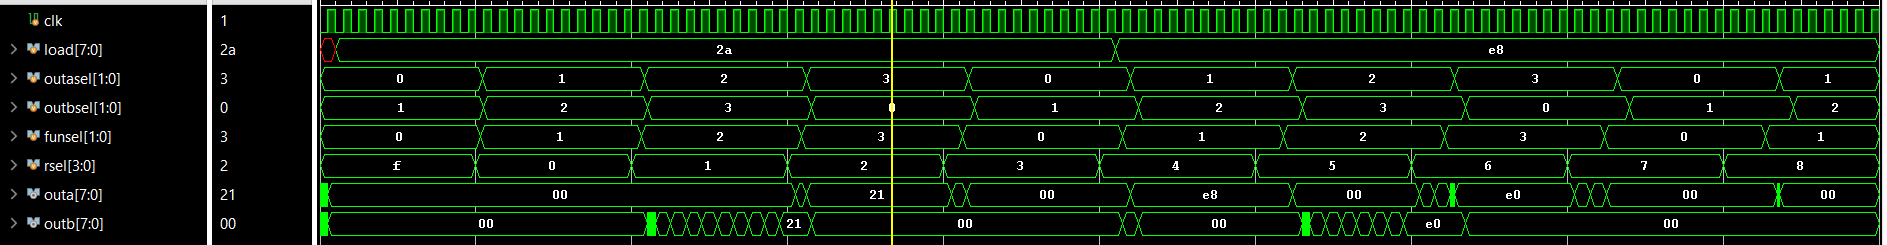
\includegraphics[width=1\textwidth]{results/arf.png}	
	\caption{ARF Simulation}
	\label{ARF Simulation}
\end{figure}

\subsection{Part 3}
\begin{figure}[H]
	\centering
	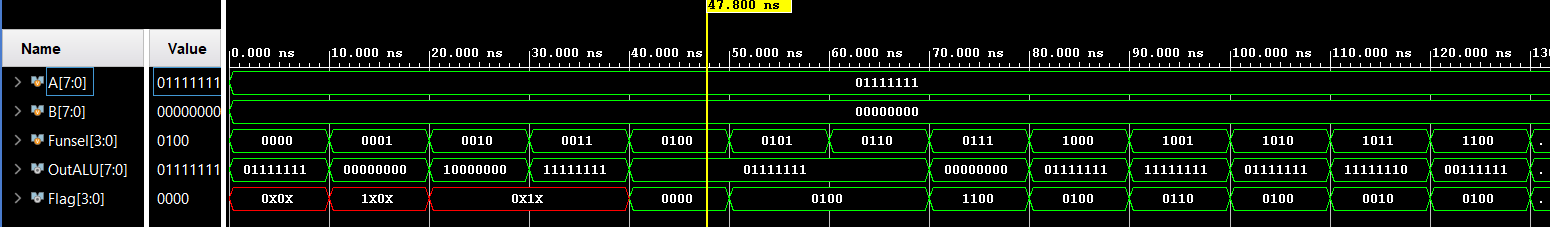
\includegraphics[width=1\textwidth]{results/alu_1.png}	
	\caption{ALu Simulation, First Image}
	\label{ALU Simulation 1}
\end{figure}
\begin{figure}[H]
	\centering
	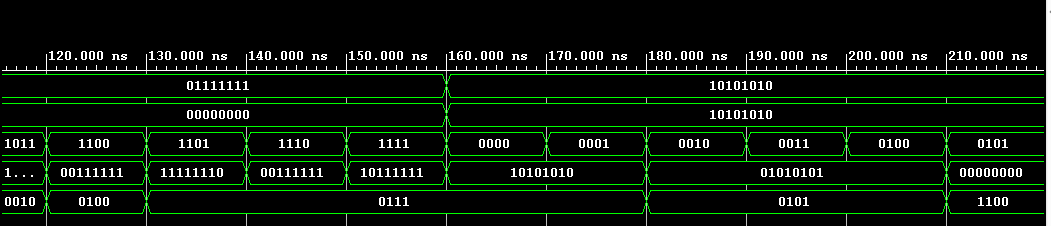
\includegraphics[width=1\textwidth]{results/alu_2.png}	
	\caption{ALu Simulation, Second Image}
	\label{ALU Simulation 2}
\end{figure}
\begin{figure}[H]
	\centering
	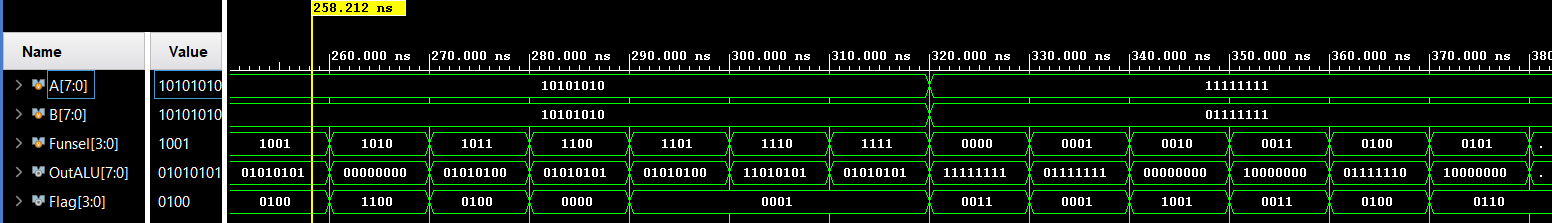
\includegraphics[width=1\textwidth]{results/alu_3.png}	
	\caption{ALu Simulation, Third Image}
	\label{ALU Simulation 3}
\end{figure}
\begin{figure}[H]
	\centering
	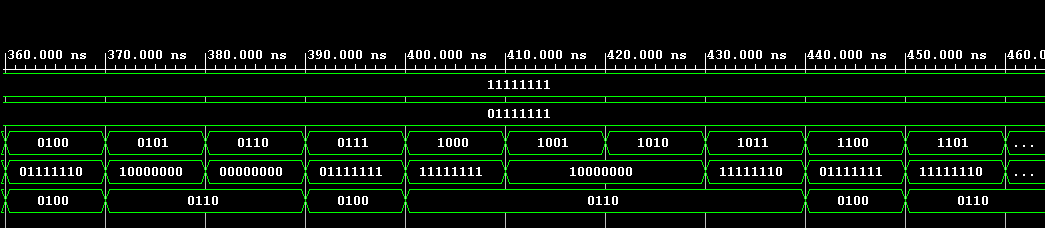
\includegraphics[width=1\textwidth]{results/alu_4.png}	
	\caption{ALu Simulation, Fourth Image}
	\label{ALU Simulation 4}
\end{figure}

\subsection{Part 4}
result of the part 4 is still contreversial so we will wait for it.


\section{CONCLUSION}

\end{document}

